% Optional appendix insert. Conditional rows include every nonempty gold bin.
\begin{figure}[p]
  \centering
  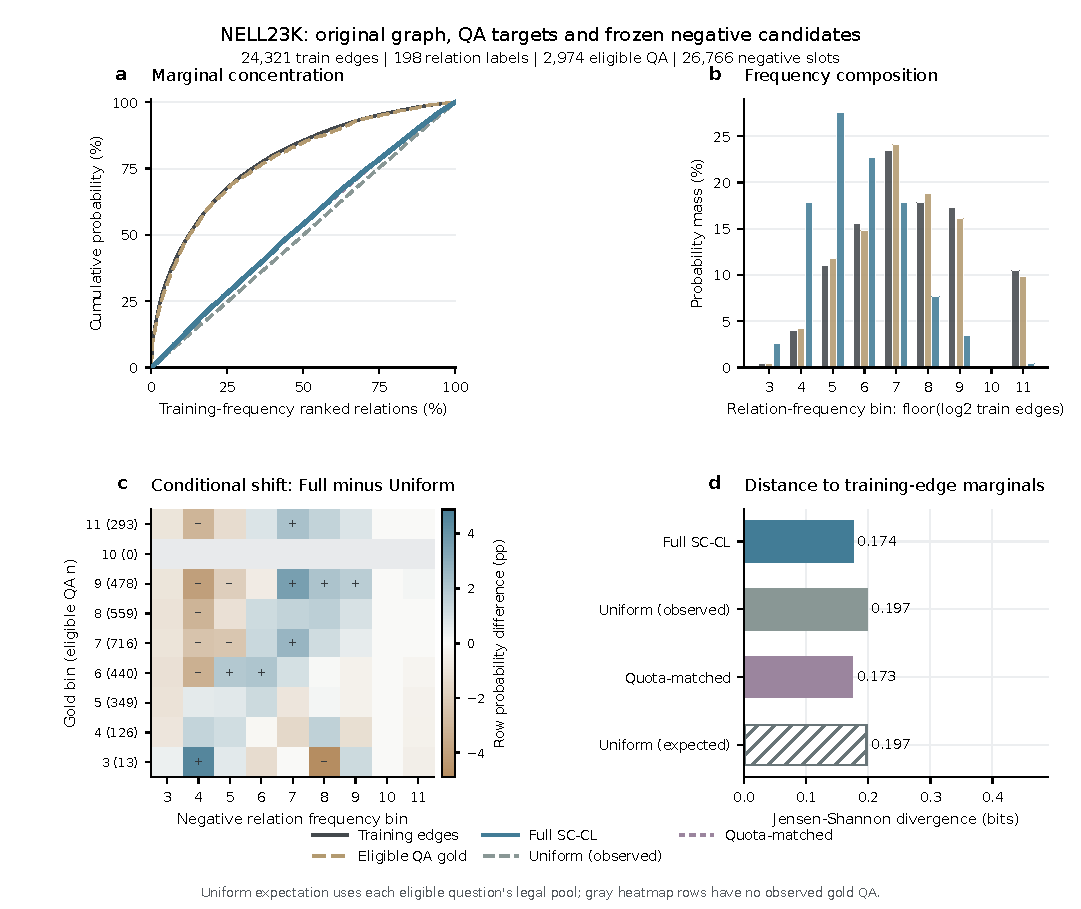
\includegraphics[width=\linewidth]{figures/sampling_distribution_seed2026/distribution_nell23k.pdf}
  \caption{NELL23K采样分布：24,321条训练边、198个关系标签、2,974道合格训练QA与26,766个Full负候选槽位。a，固定训练频次排序的累积分布；b，训练频次的$\lfloor\log_2 f(r)\rfloor$桶质量；c，在相同gold频率桶内，Full负候选桶比例减去合法池Uniform解析期望，单位为百分点，每行归一化，纵轴括号为QA数；灰色为无观测gold桶，正负符号标出绝对值不低于本面板最大值35\%的差异；d，到训练边关系分布的JS散度。条件桶样本数不同，较大色差不代表统计显著。}
  \label{fig:sampling-nell}
\end{figure}

\begin{figure}[p]
  \centering
  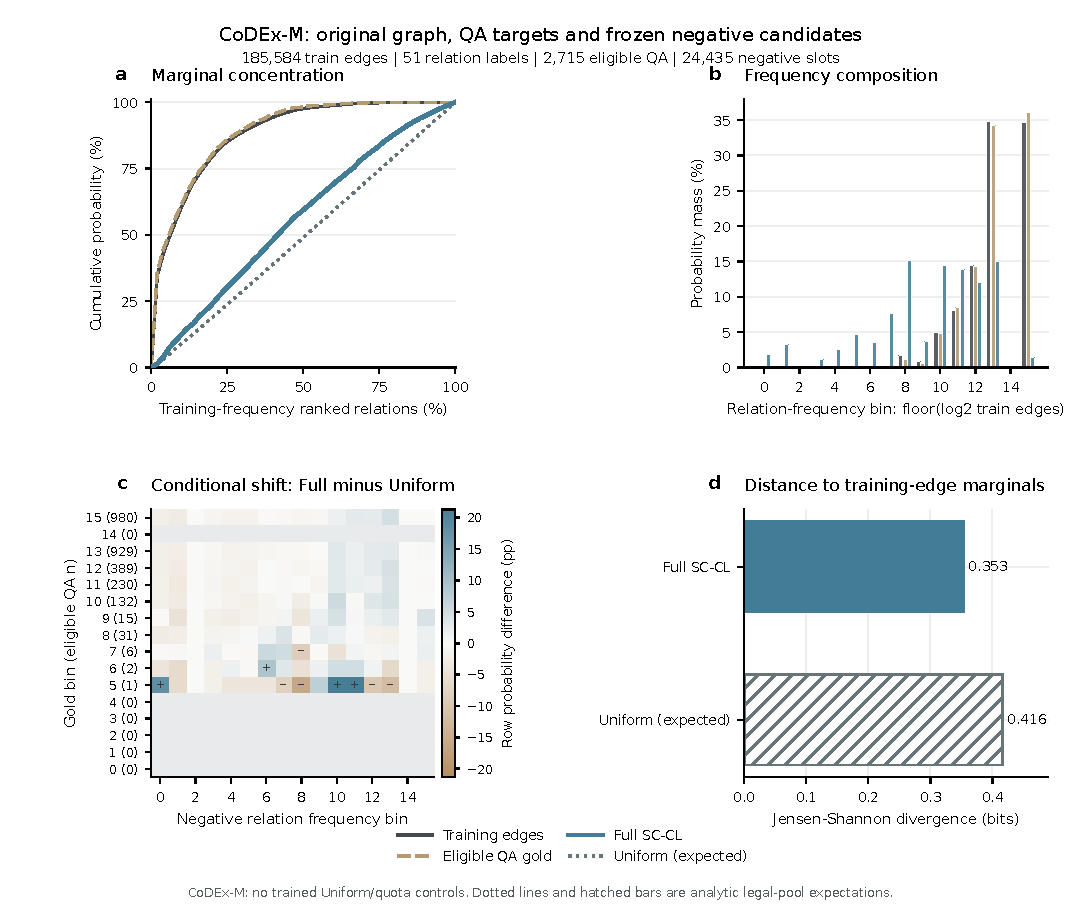
\includegraphics[width=\linewidth]{figures/sampling_distribution_seed2026/distribution_codexm.pdf}
  \caption{CoDEx-M采样分布：185,584条训练边、51个关系标签、2,715道合格训练QA与24,435个Full负候选槽位。面板定义同图~\ref{fig:sampling-nell}。该数据集未运行匹配Uniform或配额控制；点线与斜线柱仅表示逐题合法池均匀解析期望。热图使用所有非空gold桶，并标出各桶QA数；稀少问题形成的条件差异不用于机制或显著性推断。}
  \label{fig:sampling-codexm}
\end{figure}

\begin{figure}[p]
  \centering
  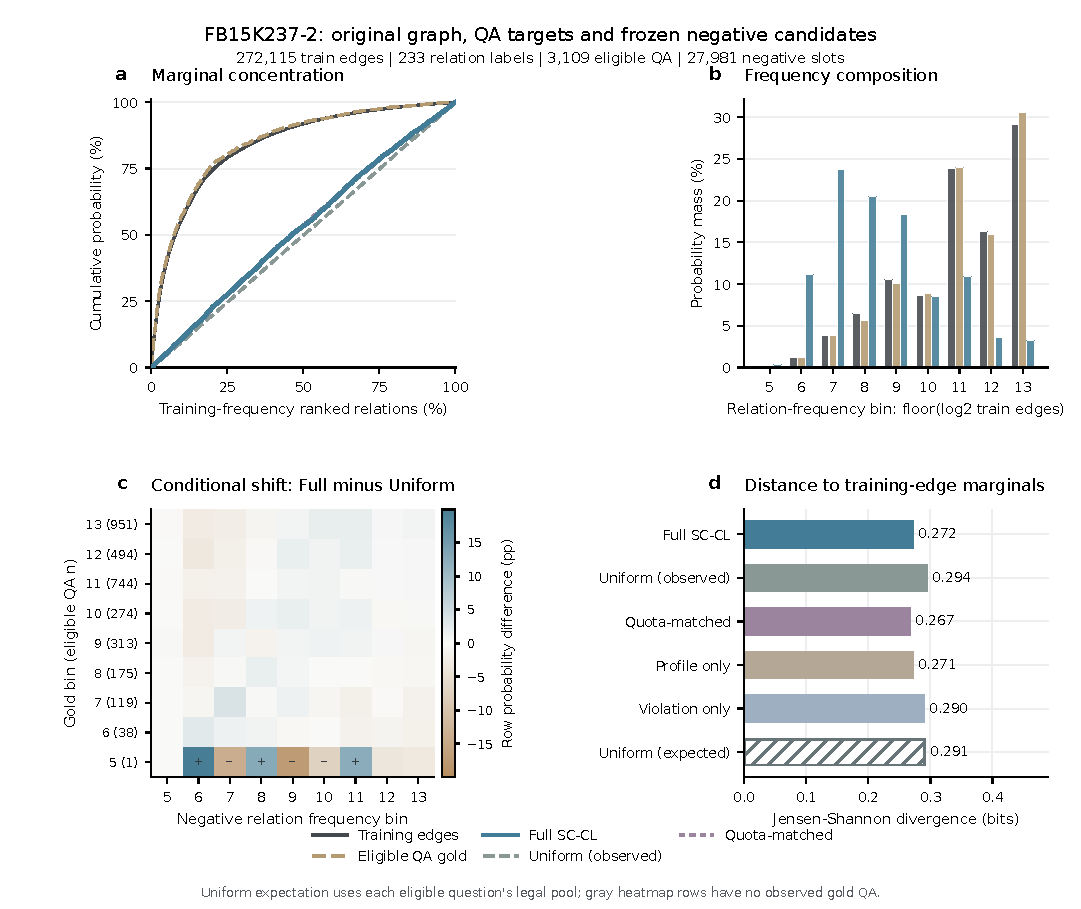
\includegraphics[width=\linewidth]{figures/sampling_distribution_seed2026/distribution_fb15k237_2.pdf}
  \caption{FB15K237-2采样分布：272,115条训练边、233个映射后关系标签、3,109道合格训练QA与27,981个Full及独立频次比例组负候选槽位；原始训练关系ID为237个。面板定义同图~\ref{fig:sampling-nell}；a、b、d另显示独立训练频次比例采样。其实际负候选边缘分布到训练边分布的JS散度为0.003，Full为0.272；分布接近不代表预测性能更高，该组直接EM为70.57\%。c仍显示Full相对合法池Uniform的条件频率桶差异；d同时保留两个单信号控制。Full与配额匹配组逐题频率桶配额相同，但具体关系可不同。}
  \label{fig:sampling-fb}
\end{figure}

\begin{figure}[p]
  \centering
  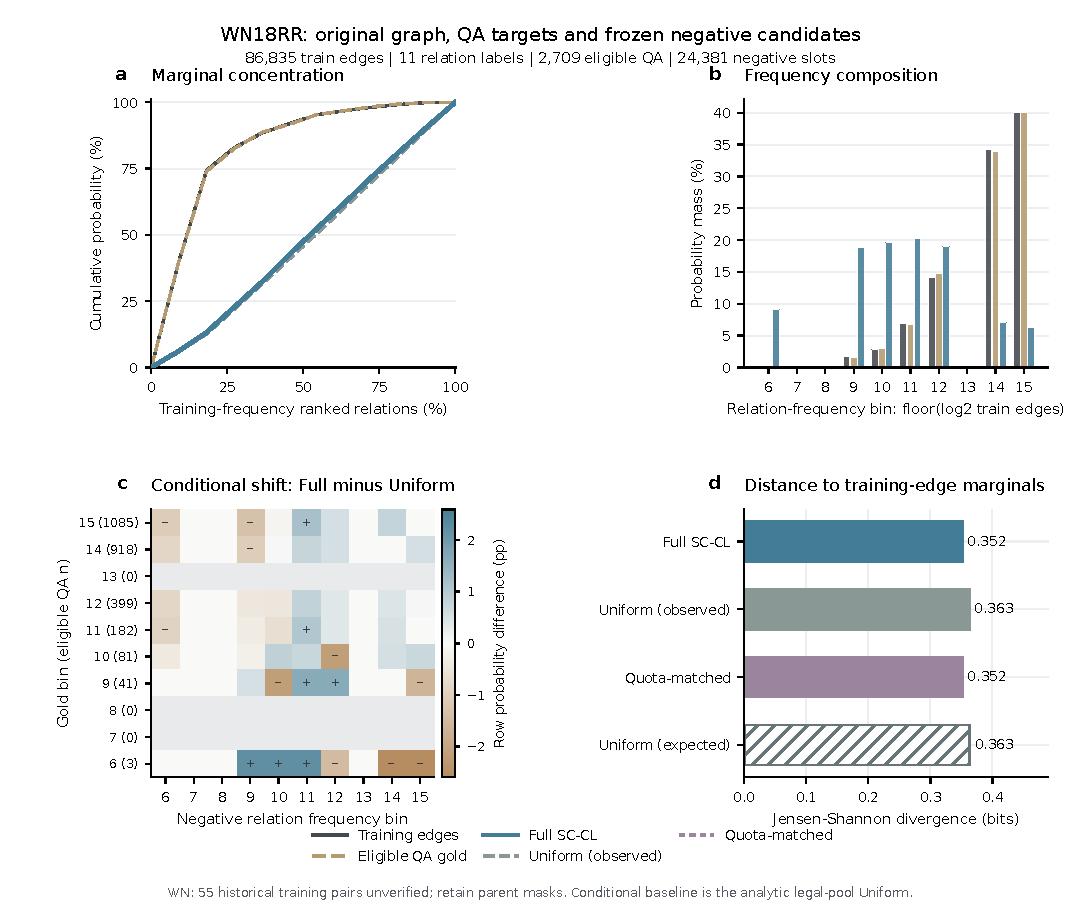
\includegraphics[width=\linewidth]{figures/sampling_distribution_seed2026/distribution_wn18rr.pdf}
  \caption{WN18RR采样分布：86,835条训练边、11个关系标签、2,709道合格训练QA与24,381个Full负候选槽位。面板定义同图~\ref{fig:sampling-nell}。55条历史训练QA实体对未独立核实，沿用原排除mask；本图为历史池条件分析，不表示全部train-pair过滤已核验。排除这55条后，Full到训练边分布的JS散度为0.3520，与全体0.3516接近；两种Full边缘分布的TV为0.00078，该敏感性检查不能修复原核验缺口。}
  \label{fig:sampling-wn}
\end{figure}
